\section{Hypothesis and Implement} %6.2
Referencing Figure~\ref{4_1_1_without2} in Subsection~\ref{subsection4.1.1}, we find one of the lowest points to simulate one of the worst situation we can find in Noridc system, as shown in the Figure~\ref{6_2_g9}, as our start point of Emergency Control.

\begin{figure}[htbp]
\centering
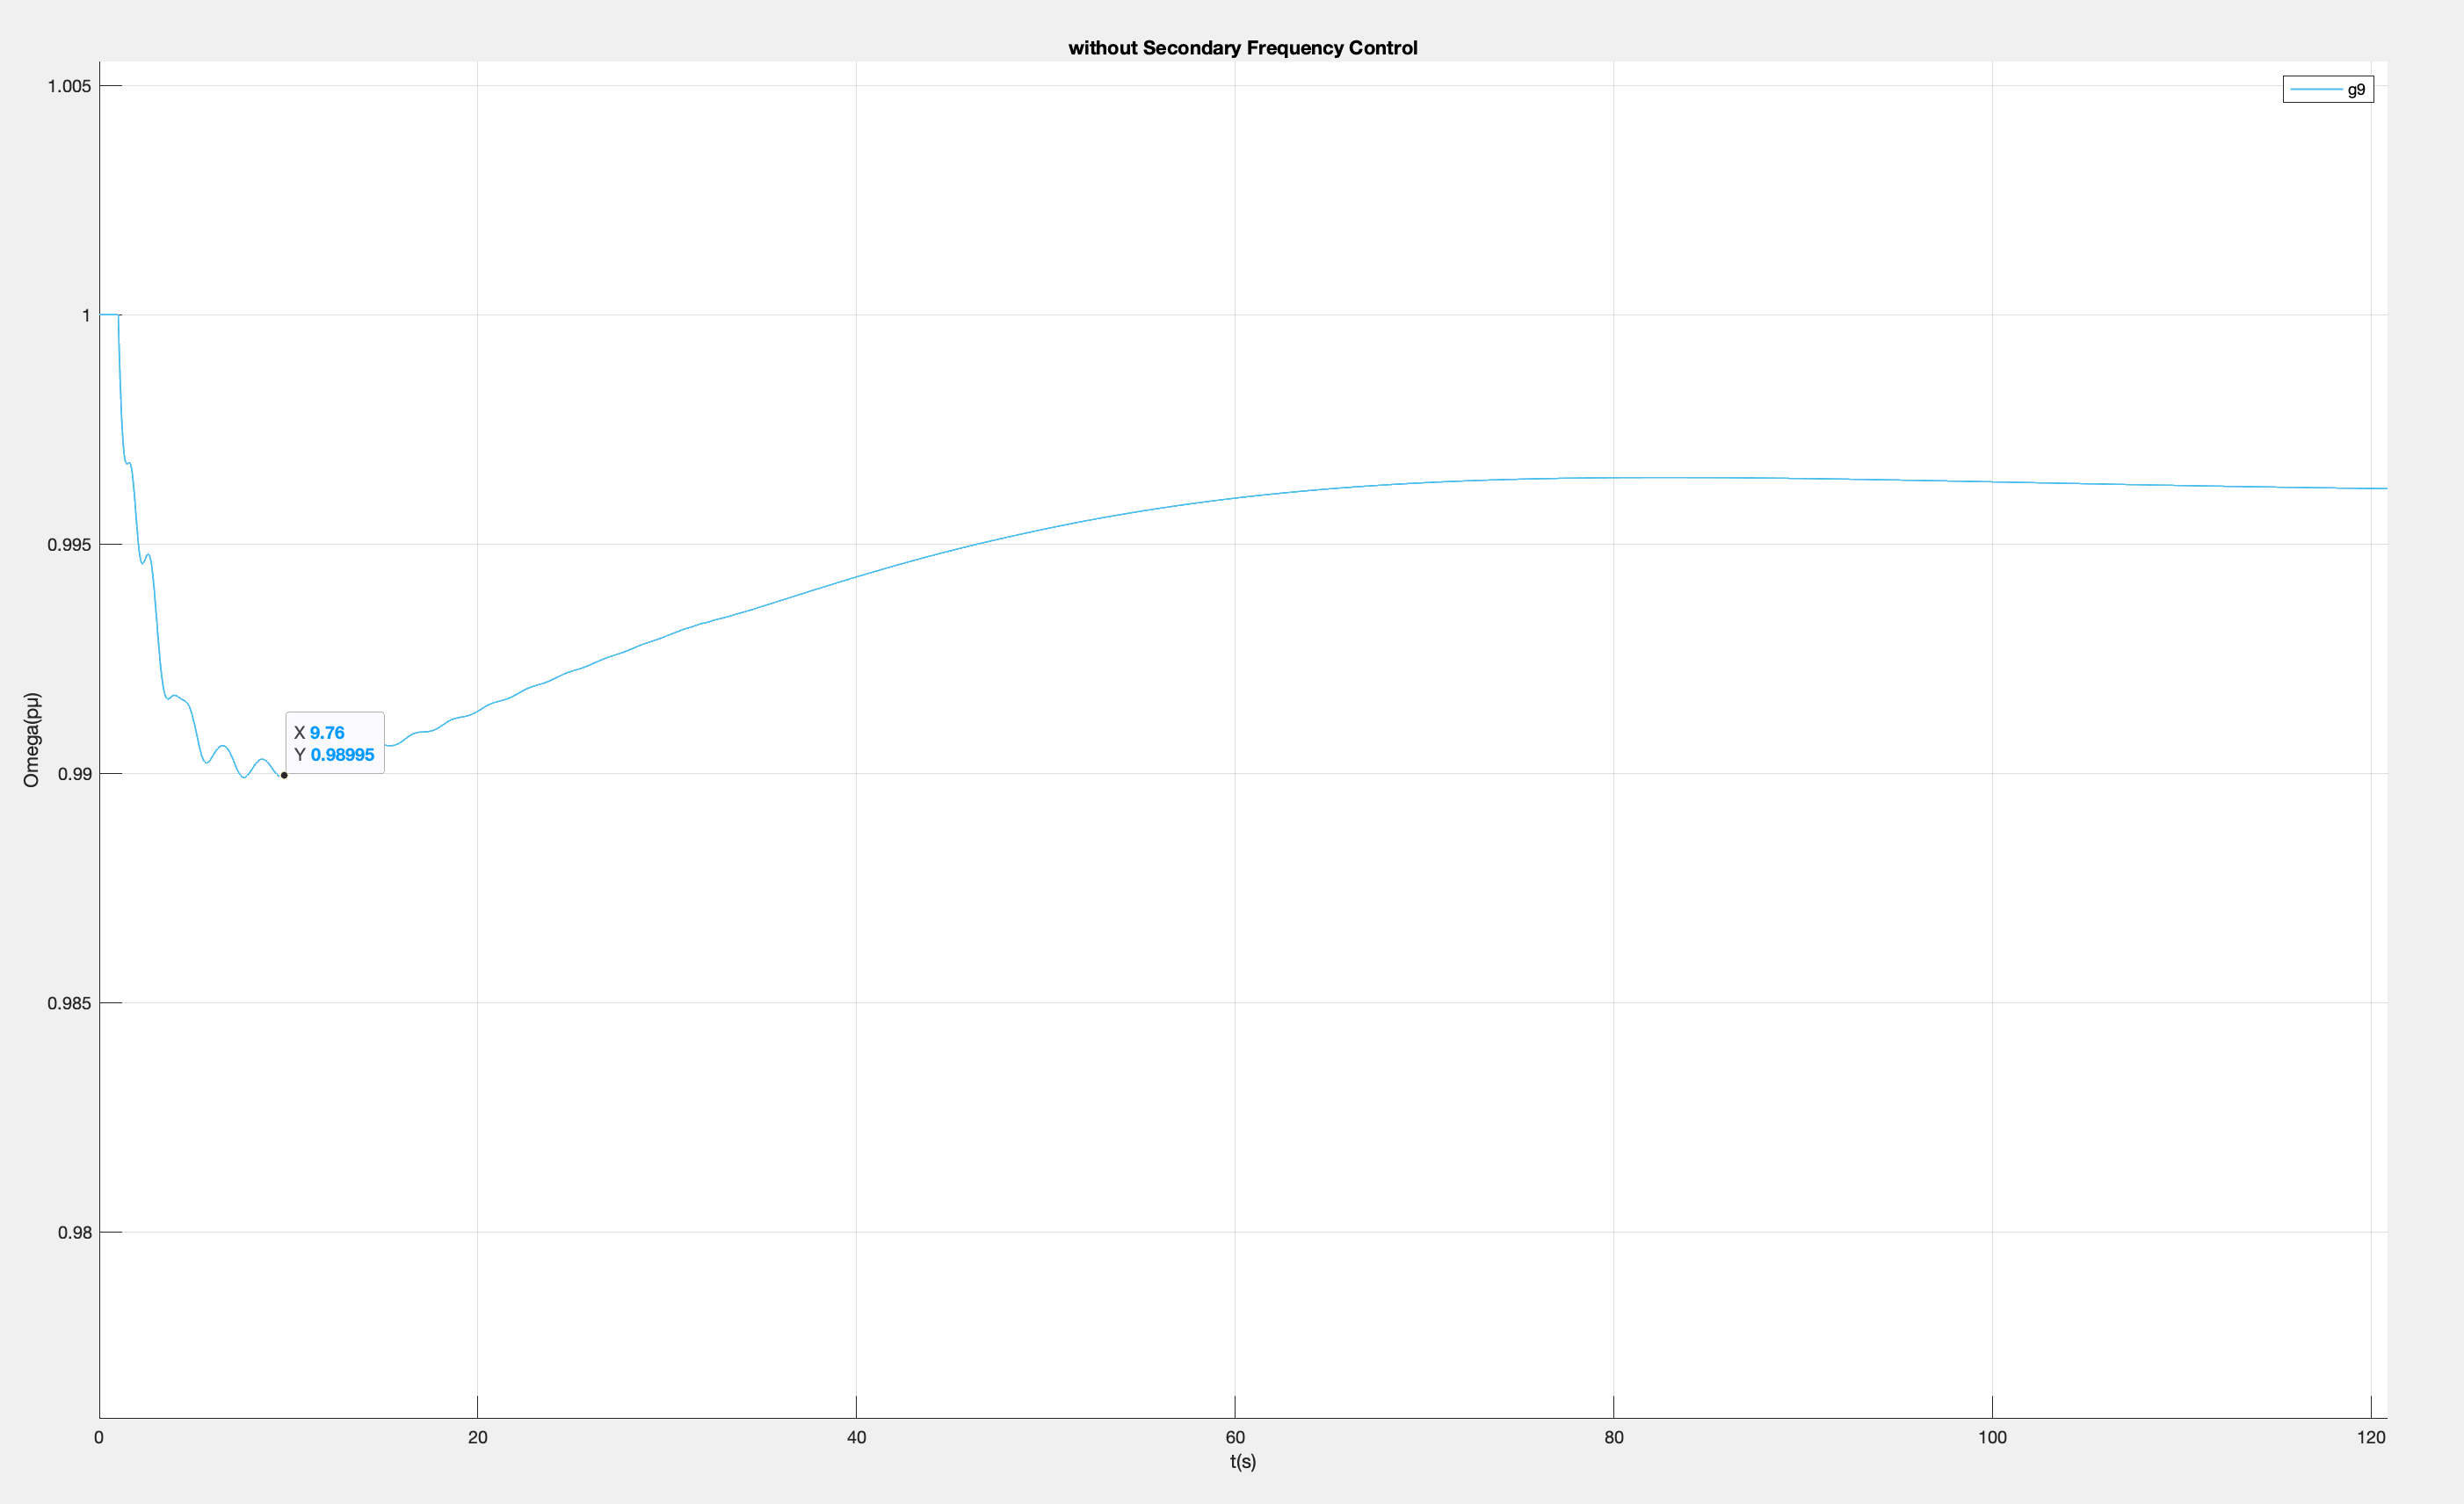
\includegraphics[width = .819\textwidth]{figure/6_2_g9.png}
\caption{Start time of Emergency Control.}
\label{6_2_g9}
\end{figure}

We start the Emergency Control from the 9.76th second and tuned kp, ki and time delay, i.e. kp is from 0.1 to 140.1 (step is 10.0), ki is from 0.1 to 10.1 (step is 1.0) and time delay is from 0.01 seconds to 0.21 seconds (step is 0.01sec), which are the same tuning conditions in Chapter~\ref{Chapter5}. The aim of such hypotheses is to test the impact of time delay under the condition of Emergency Control and compare the simulation results with SFC. The simulation lasts for 1000 seconds. 